\documentclass[12pt,oneside,openany,titlepage,letterpaper]{wmthesisMod}  %Use these options for official University copies
%\documentclass[12pt,oneside,openany,titlepage,letterpaper]{wmthesis-arjun}  %Use these options for official University copies

%%%%%%%%%%%%%%%%%%%%%%%%%%%%%%%%%%%%%%%%%%%%%%%%%%%%%%%%%%%%%%%%%%%%%%%%%%
%=========================================================================
% Include Extra Packages Here
%
% Use the Hypertex References package (if doing PDF)
%\usepackage{hyperref}
%
% Use the Vpage package which creates the proper
% Page Layout (USletter, USlegal, etc...)
% see pages 88-89 of The LaTeX companion
%\usepackage{Vmargin}
%
% Use the doublespace package for linespacing
%\usepackage{doublespace}
% ERROR: This package is not compatible with color! <wirawan0>
% Don't use that! We implicitly call the newer `setspace' package in
% the main `wmthesis' style.
%
% Use both the AMS math and symbols packages
% for equations
\usepackage{amsmath}
\usepackage{amssymb}
% for \bm math bold symbol macros, if you want them:
\usepackage{bm}
\usepackage{cite}
%
% Set the font family to use for the thesis
%
% \usepackage{times,mathptmx}
%
% Wirawan's default font selections: we use Times Roman for the text,
% but Computer Modern for the math (nicer). Remove the following 3 TeX
% lines if you don't like the appearance.
% - roman     : Times
% - sans serif: Computer Modern Sans Serif
% - typewriter: Computer Modern Typewriter
%%\renewcommand{\rmdefault}{ptm}
%%\renewcommand{\sfdefault}{cmss}
%%\renewcommand{\ttdefault}{cmtt}
% LaTeX-level hacks
% Euler, roman, medium (for walker indices)
\DeclareMathAlphabet{\matheurm}{U}{eur}{m}{n}
%
% [wirawan0] Using colors whenever appropriate:
%
\usepackage{color}
%
% [wirawan0] Use customizable bibliography citation
%
\usepackage[square,numbers,compress]{natbib}
%
% Use the standard Graphicx Package
% for graphics inclusion with the dvips driver
%\usepackage[dvips]{graphicx}
\usepackage{graphicx}
\graphicspath{{./figs}{.}}
%
% Use the EPS figure package for including
% encapsulated postscript figures
%\usepackage{epsfig}
%\usepackage{psfig}
%
% Use the standard Postscript Tricks package
% for graphics inclusion with the dvips driver
% \usepackage{pstricks,pst-node,pst-text}
%
% Use the PSFrag package for PS text replacement
% \usepackage{psfrag}
%
% Use the TextCase package for special text caps
% \usepackage{textcase} -- see wmthesis
%
% Use the Xspace package for proper spacing
% after macros
% \usepackage{xspace}
%
% Use the Subfigure package to create arrays of
% figures
% \usepackage{subfigure}
%
% Use the Calc package for integer opps
% \usepackage{calc}
%
% Use the TabularX package to create special tables
% \usepackage{tabularx}
%
% Use the enumerate package for custom lists
\usepackage{enumerate}


%
% use the Dcolumn package to allow for aligned columns
% in tables
\usepackage{dcolumn}
%
% Use the MakeIndex Package to generate an index
%
\usepackage{makeidx}




%
% Use the Afterpage Package to flush out unprocessed floats
%
% \usepackage{afterpage}
%
% Use fancy if-then-else logic on some of my macros:
%
\usepackage{ifthen}
%
% Use `programmable' inline drawings: uncomment if you want them
%
%\usepackage{texdraw}
%\input{txdtools.tex}
%
% Set the Paper Size to Letter
%\setpapersize{USletter}
%
% Set Up the margins to use
%\setmarginsrb{1in}{1in}{1in}{1in}{0pt}{10mm}{0pt}{5mm}
%
%%%%%%
% Include your macro files here
% This includes any redefinition of commands or environments
%%%%%%%%%%%%%%%%%%%%%%%%%%%%%%%%%%%%%%%%%%%%%%%%%%%%%%%%%%%%%%%%%%%%%%%%%%
%
% Ph.D. dissertation manuscript
% Global LaTeX macros
%
% Brad Student (January 2005)
% College of William and Mary
% Department of Physics
% Prof. Sharp Mind, advisor
%
% $Id: Diss-title.tex,v 1.5 2005/01/14 22:32:00 wirawan Exp $
%
% Based on Paul King and Andrew Norman's template (modified)
%
%%%%%%%%%%%%%%%%%%%%%%%%%%%%%%%%%%%%%%%%%%%%%%%%%%%%%%%%%%%%%%%%%%%%%%%%%%

% Simple equation macros (note how the align or align* environment is used
% in AMS-math documentation, if you're going to use this).
\newcommand\eq[1]                              % single unlabeled equation
{
\begin{align*}
#1
\end{align*}
}

\newcommand\eql[2] % single labeled equation
{
\begin{equation}\label{#1}
\begin{split}
#2
\end{split}
\end{equation}
}

\newcommand\eqnl[2]        % single labeled equation (maunya sih, centered
{%                     equation array dg satu label saja (apakah bisa???))
\begin{equation}\label{#1}
%\begin{split}
#2
%\end{split}
\end{equation}
}

% WARNING: eqsl is REDEFINED!
\newcommand\eqsl[1]                            % multiply labeled equation
{
\begin{align}
#1
\end{align}
}

\newcommand\eqssl[2]                      % multiply labeled SUB-equations
{
\begin{subequations}\label{#1}
\begin{align}
#2
\end{align}
\end{subequations}
}

% FORMATTING SHORTCUTS:
\newcommand\prg[1]     {\texttt{#1}}                   % computerish stuff

% Formatting for captions:
% Usage:
% \xcaption{Label}{First caption included in TOC.}{More caption text.}
% or
% \xcaption[Caption for TOC.]{Label}{First caption text.}{More caption text.}
\newcommand\xcaption[4][] {
    \ifthenelse{\equal{#1}{}}
               {\caption[#3]{\label{#2}#3 #4}}
               {\caption[#1]{\label{#2}#3 #4}}
}
% The following is needed because caption is too close to the table:
\newcommand\TableCaptionSkip {\vskip 0.4cm}
% Table caption: similar to \xcaption above
\newcommand\tcaption[4][] {
    \xcaption[#1]{#2}{#3}{#4}
    \TableCaptionSkip
}
% Autocentering for graphics:
\newcommand\IncludeGraphics[2][] {
    \begin{center}
    \includegraphics[#1]{#2}
    \end{center}
}
\newcommand\FIGURE[1]  {figures/#1}     % -- if specific-plotdir is wanted

% Referencing shortcuts:
\providecommand\eqref[1] {(\ref{#1})}  %if your stylesheet doesn't have it
\newcommand\Appendix[1]{Appendix~\ref{#1}}
\newcommand\Chapter[1] {Chapter~\ref{#1}}
\newcommand\ChapSec[2] {Chapter~\ref{#1}, \Sec{#2}}
\newcommand\Eq[1]      {Eq.~\eqref{#1}}
\newcommand\Eqs[1]     {Eqs.~\eqref{#1}}
\newcommand\Fig[1]     {Fig.~\ref{#1}}
\newcommand\Sec[1]     {Sec.~\ref{#1}}
\newcommand\Ref[1]     {Ref.~\onlinecite{#1}}
\newcommand\Refs[1]    {Refs.~\onlinecite{#1}}
\newcommand\Cite[1]    {~\cite{#1}}                % user-modifiable \cite

% Coloring and marking
\definecolor{Red}{rgb}{0.8,0.2,0.2}%red
\definecolor{Green}{rgb}{0.08,0.60,0.08}%green
\definecolor{Blue}{rgb}{0.3,0.3,1.0}%blue
\definecolor{dkBlue}{rgb}{0.1,0.1,0.5}%dark blue
\definecolor{Black}{rgb}{0,0,0}
\definecolor{Gold}{rgb}{0.60,0.60,0.08}%gold-like color
\definecolor{Remarks}{rgb}{1,0.3,0.3}%red
\definecolor{Extra}{rgb}{0.2,0.2,1}%blue

% DRAFTING utility
\newcommand\COMMENTED[1] {}

% KE - added following Macros
\newcommand\ket[1]     {|{{#1}}\rangle}
\newcommand\bra[1]     {\langle{{#1}}|}

\newcommand\REMARKS[1]   {\textbf{\textcolor{Red}{[#1]}}}
%\newcommand\REMARKS[1]   {}
\newcommand\REMARKSBLUE[1]   {\textbf{\textcolor{Blue}{[#1]}}}
% You are certainly welcome to customize the macros above (or erase the
% ones that you don't like). Add your own macros here, too.
                      % Locate your macros here
%
% If you are indexing include the \makeindex
% command here and run an index pass
%\makeindex                             % Generate an index
%
%=========================================================================
%%%%%%%%%%%%%%%%%%%%%%%%%%%%%%%%%%%%%%%%%%%%%%%%%%%%%%%%%%%%%%%%%%%%%%%%%%





% Begin the Text of the Main Document
\begin{document}                        % Begin the documentz
%\input{Thesis_Margin_Marks}            % Overlay the Margins for the Thesis
\normalsize                             % Return to Normal font size
\begin{spacing}{2.0}                    % Double Space the Text

\frontmatter
%%%%%%%%%%%%%%%%%%%%%%%%%%%%%%%%%%%%%%%%%%%%%%%%%%%%%%%%%%%%%%%%%%%%%%%%%%
%
% Ph.D. dissertation manuscript
% Title page
%
% Brad Student (January 2005)
% College of William and Mary
% Department of Physics
% Prof. Sharp Mind, advisor
%
% $Id: Diss-title.tex,v 1.5 2005/01/14 22:32:00 wirawan Exp $
%
% Based on Paul King and Andrew Norman's template (modified)
%
%%%%%%%%%%%%%%%%%%%%%%%%%%%%%%%%%%%%%%%%%%%%%%%%%%%%%%%%%%%%%%%%%%%%%%%%%%


%%%%%%%%%%%%%%%%%%%%%%%%%%%%%%%%%%%%%%%%%%%%%%%%%%%%%%%%%%%%%%%%%%%%%%%%%%
\title{An Informative and Brief Title}
% Set the subtitle if you need to. Comment the following line if you don't
% want any subtitle (most of the students DON'T WANT subtitle):
%\subtitle{The New Way to Understand Physics}

\author{ Ima Grad Student }
\hometown{Williamsburg, Virginia}
\prevdeg{
Master of Science, College of William \& Mary, 2015\\  %% Modify this part to fit your educational background.
Bachelor of Science, Random University, 2013}
\graduationmonth{August 2019} % Month and Year degree is conferred
\copyyear{2019} % Year of copyright

% Committee members
% The first one must be your own advisor (the word "Chair" will be added
% automatically)
\cmtyA{Professor Jane Doe, Physics}
% Sort the name of the rest of the committee members by their last name
% The external member must be put last. If he/she is from W&M, then
% the institution name "College of William and Mary" is not needed, the
% department name is sufficient.
\cmtyB{\parbox{5in}{\renewcommand{\baselinestretch}{1.0}%\small\normalsize%
                    \center Professor Generic Name, Physics \\ \vskip -0.13in %nbp added vskip
		    College of William \& Mary}}
\cmtyC{\parbox{5in}{\renewcommand{\baselinestretch}{1.0}%\small\normalsize%
                    \center Assistant Professor Generic Name, Physics \\ \vskip -0.13in %nbp added vskip
		    College of William \& Mary}}
\cmtyD{\parbox{5in}{\renewcommand{\baselinestretch}{1.0}%\small\normalsize%
                    \center Professor Another Person, Physics \\ \vskip -0.13in %nbp added vskip
		    College of William \& Mary}}
\cmtyE{\parbox{5in}{\renewcommand{\baselinestretch}{1.0}%\small\normalsize%
                    \center Dr. External Person, Physics\\ \vskip -0.13in %nbp added vskip
		    Institute of Advanced Research}}

%%%%%%%%%%%%%%%%%%%%%%%%%%%%%%%%%%%%%%%%%%%%%%%%%%%%%%%%%%%%%%%%%%%%%%%%%%
\maketitle[\@graduationmonth]
\makeapproval[Approved by the Committee July 2019] % Month and Year of defense
\pagenumbering{roman}
%\makeapproval[Draft Version, \monthyear]  % Just remove this argument for
%                                          % the final version.
%%%%%%%%%%%%%%%%%%%%%%%%%%%%%%%%%%%%%%%%%%%%%%%%%%%%%%%%%%%%%%%%%%%%%%%%%
                       % Include the title page and approval page

\begin{abstract}
\begin{flushleft}
%%%%%%%%%%%%%%%%%%%%%%%%%%%%%%%%%%%%%%%%%%%%%%%%%%%%%%%%%%%%%%%%%%%%%%%%%%
%
% Ph.D. dissertation manuscript
% Dissertation abstract
%
% Brad Student (January 2005)
% College of William and Mary
% Department of Physics
% Prof. Sharp Mind, advisor
%
% $Id: Diss-vita.tex,v 1.4 2005/01/14 22:32:00 wirawan Exp $
%
% Based on Paul King and Andrew Norman's template (modified)
%
% This is to be used for BOTH the normal abstract and the UMI abstract.
%
% UMI abstract is printed as the last page of this document, but DO NOT
% include that page as the final dissertation.
% Include that separately from the three copies of the dissertation to
% the Office of the Dean of Graduate Studies.
%
%%%%%%%%%%%%%%%%%%%%%%%%%%%%%%%%%%%%%%%%%%%%%%%%%%%%%%%%%%%%%%%%%%%%%%%%%%
\thispagestyle{empty}
\noindent

This is a well written abstract.
\end{flushleft}
\end{abstract}

\pagenumbering{roman}
\tableofcontents

%%%%%%%%%%%%%%%%%%%%%%%%%%%%%%%%%%%%%%%%%%%%%%%%%%%%%%%%%%%%%%%%%%%%%%%%%%
%
% Ph.D. dissertation manuscript
% Acknowledgements
%
% Brad Student (February 2008)
% College of William and Mary
% Department of Physics
% Prof. Sharp Mind, advisor
%
% $Id: Diss-acknowledgment.tex,v 1.4 2005/01/14 22:31:59 wirawan Exp $
%
% Based on Paul King and Andrew Norman's template (modified)
%

%%%%%%%%%%%%%%%%%%%%%%%%%%%%%%%%%%%%%%%%%%%%%%%%%%%%%%%%%%%%%%%%%%%%%%%%%%

%added /normalfont, /large to match other titles and standard TSH
\chapter*{\normalfont\large ACKNOWLEDGMENTS}
\addcontentsline{toc}{chapter}{Acknowledgments}
\vspace{-1.3cm} %one line between title and body, TSH
\begin{spacing}{1.0}
% 2013 standard requires this to be single-spaced, left-aligned (instead of justified, ew), no indent, and with spaces between paragraphs. TSH

\flushleft{\noindent
I acknowledge the guidance of my advisor, and everyone else that directly assisted me in my research.
\newline \\
I thank the committee members for the time and attention that they have each put in to reviewing this dissertation.
\newline \\
I would also like to thank other people, for thier personal support.
}
\vspace{1ex}
\end{spacing}

%%%%%%%%%%%%%%%%%%%%%%%%%%%%%%%%%%%%%%%%%%%%%%%%%%%%%%%%%%%%%%%%%%%%%%%%%%
\newpage
\begin{spacing}{1.0}
%\chapter*{DEDICATION}%%% DEDICATION
\addcontentsline{toc}{chapter}{Dedication}
%\topskip0pt
\vspace*{\fill}
%\begin{spacing}{1.0}
%
% November 2003 guide requires this be single-spaced
%
\begin{center}

This dissertation is dedicated to something.

\vskip .8in
\end{center}
\vspace*{\fill}
\end{spacing}


\listoftables
\listoffigures

\mainmatter

%%%%%%%%%%%%%%%%%%%%%%%%%%%%%%%%%%%%%%%%%%%%%%%%%%%%%%%%%%%%%%%%%%%%%%%%%%
%
% Ph.D. dissertation manuscript
%
% College of William and Mary
% Department of Physics
%
%%%%%%%%%%%%%%%%%%%%%%%%%%%%%%%%%%%%%%%%%%%%%%%%%%%%%%%%%%%%%%%%%%%%%%%%%%

\chapter{Introduction}
\label{chp:Intro}

There is a very challenging and fundamental problem in Physics~\cite{fakeCite}.
Now, I am explaining the problem and the approaches that have been used in order to address this problem.
These approaches are not suitable in all cases.
Now I am explaining a different approach that works in a specific set of cases.

This dissertation is organized as follows.
In Chapter~\ref{chp:background}, background material is covered.
In Chapter~\ref{chp:approach}, our approach is introduced.
Chapter~\ref{chp:results} contains results obtained from our approach.
We conclude with general remarks in Chapter~\ref{chp:summary}.

%%%%%%%%%%%%%%%%%%%%%%%%%%%%%%%%%%%%%%%%%%%%%%%%%%%%%%%%%%%%%%%%%%%%%%%%%%
%
% Ph.D. dissertation manuscript
%
% College of William and Mary
% Department of Physics
%
%%%%%%%%%%%%%%%%%%%%%%%%%%%%%%%%%%%%%%%%%%%%%%%%%%%%%%%%%%%%%%%%%%%%%%%%%%

\chapter{Background}
\label{chp:background}

The background material, which is necessary to understand the rest of this dissertation, is outlined in this chapter.

\section{Topic 1}
\label{sec:topic1}

This is an important topic.

\section{Topic 2}
\label{sec:topic2}

This is also an important topic.

\begin{figure} %Fig. 1                                                                                                                                                          
\begin{center}
%\hspace{12.0mm}                                                                                                                                                                
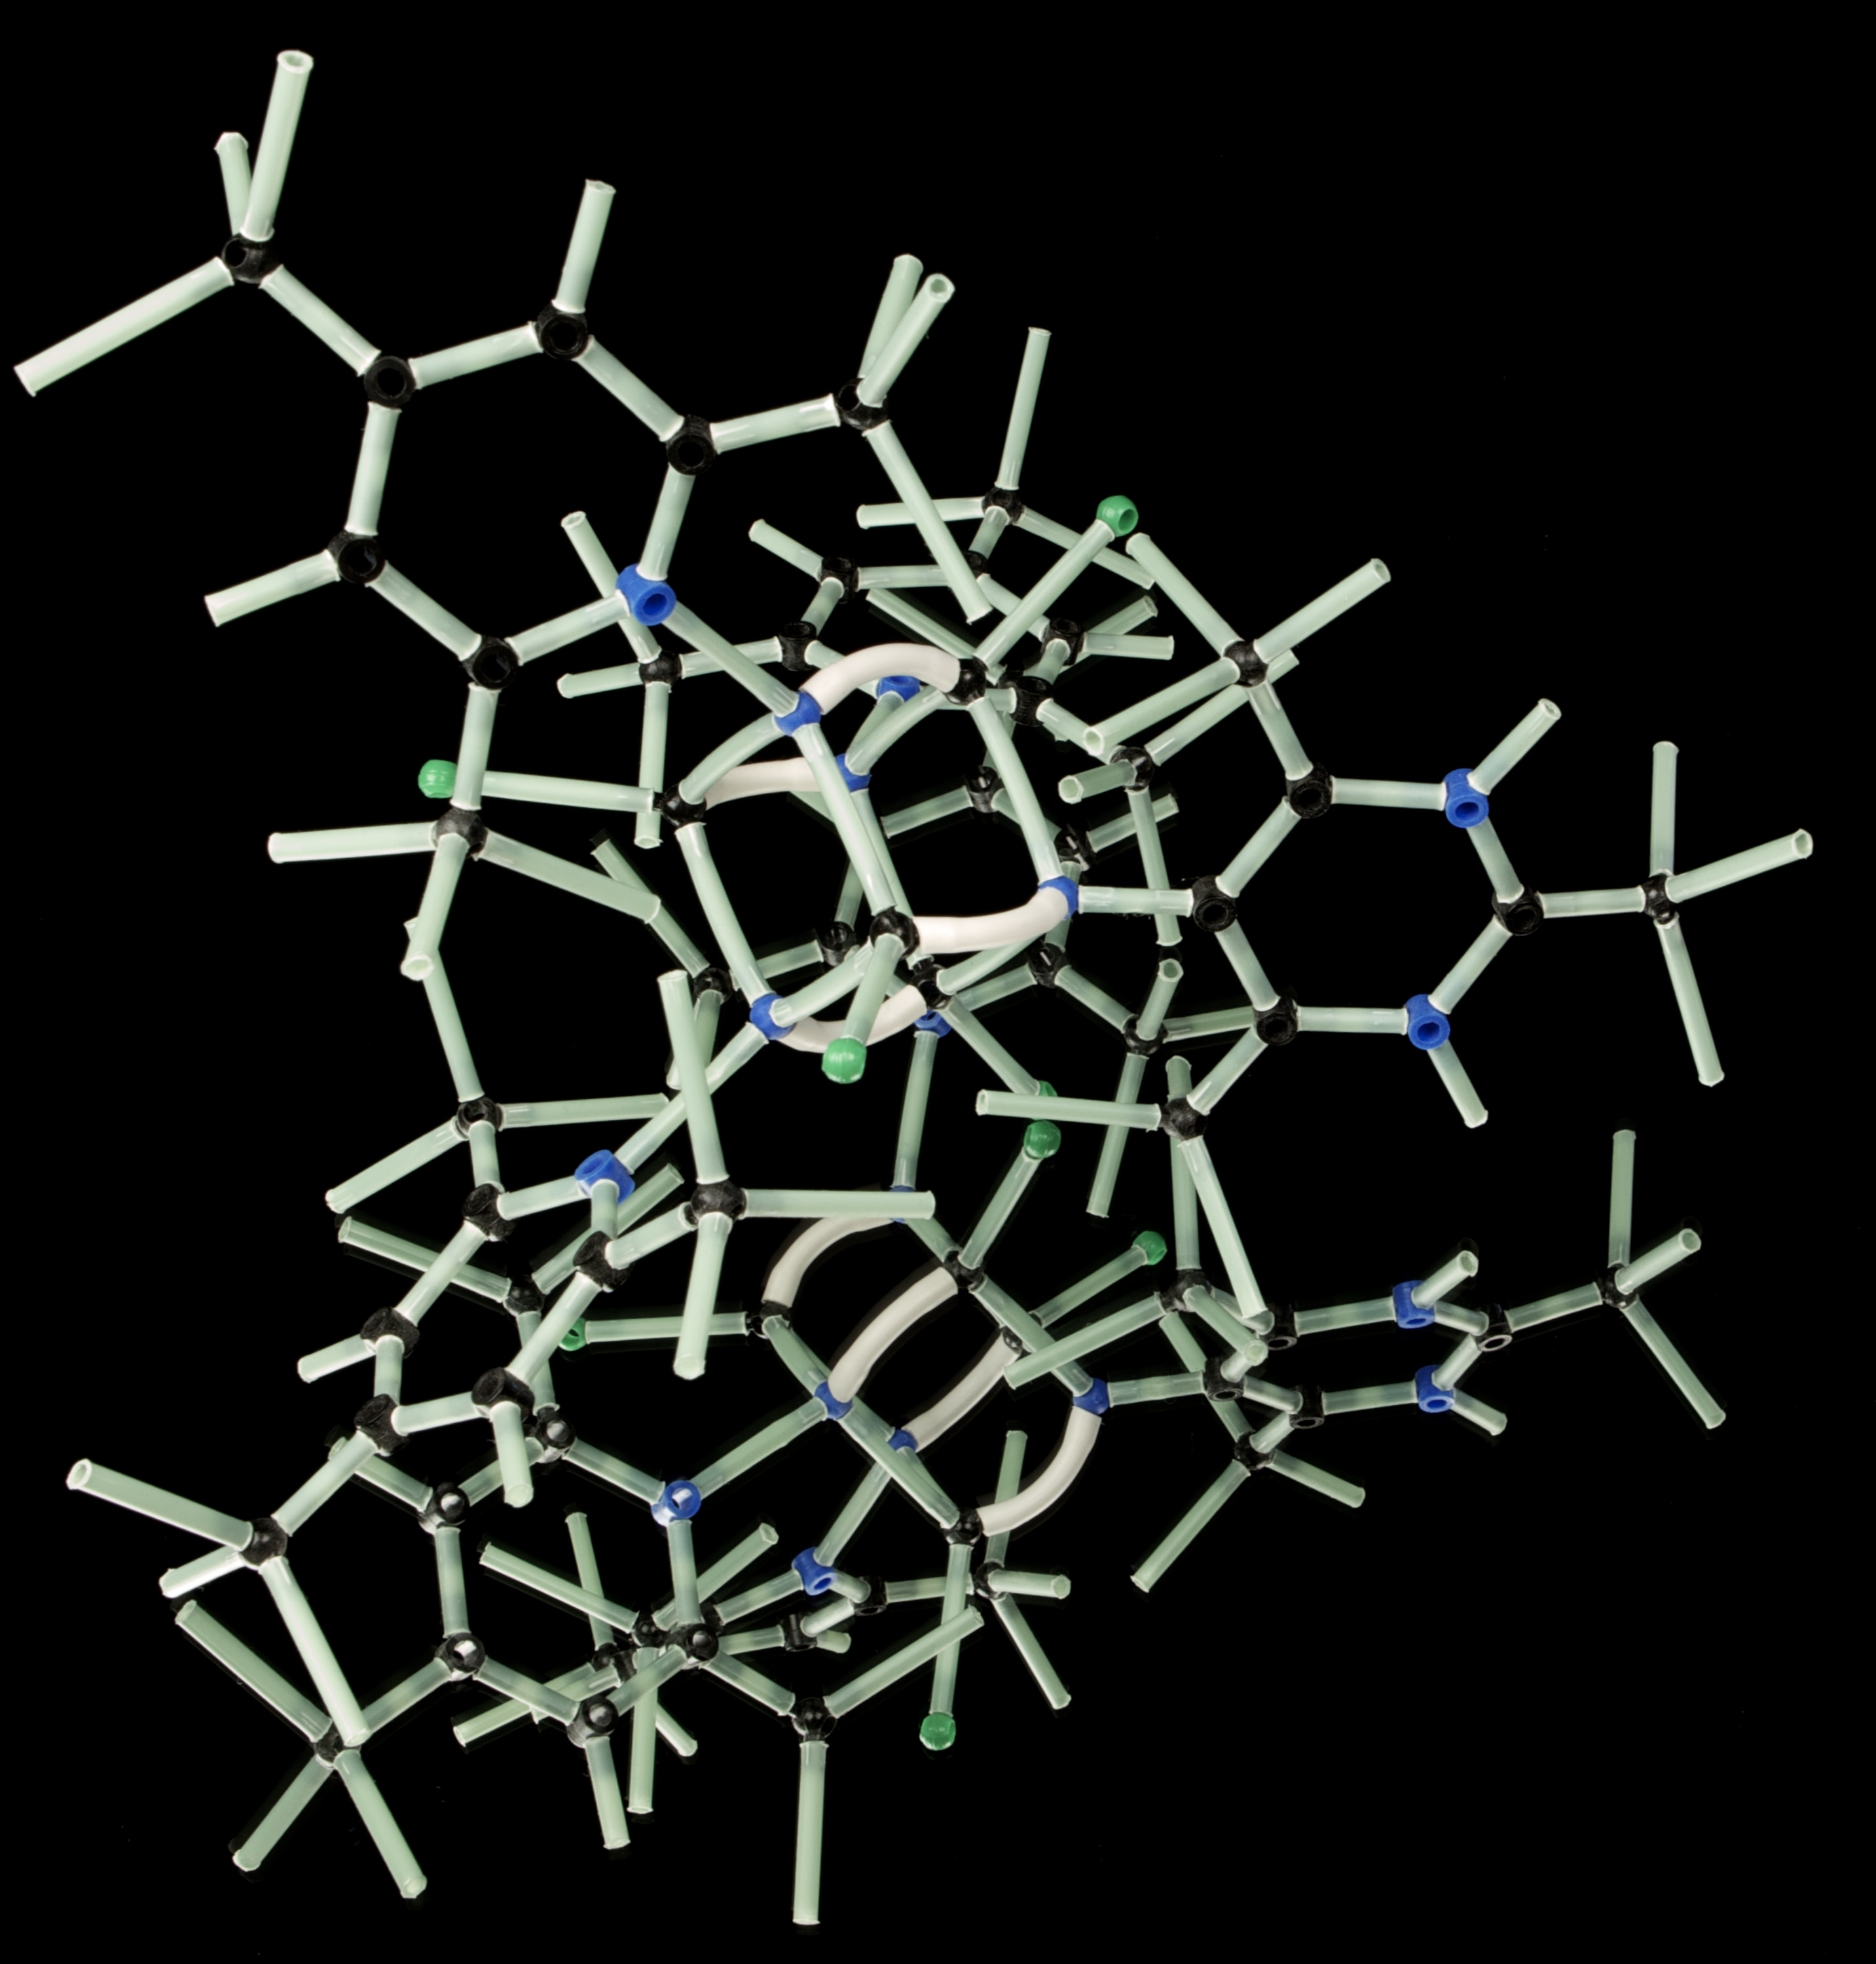
\includegraphics[width=0.6\textwidth]{figs/figure1.jpg} % use .pdf, and not .jpg. This is just an example.
\caption[a picture] % this is the short-caption that appears in the list of figures 
{\label{fig:picture}
%                                                                                                                                                                               
This is a pretty picture that helps to explain the material.
}
\end{center}
\end{figure}


%%%%%%%%%%%%%%%%%%%%%%%%%%%%%%%%%%%%%%%%%%%%%%%%%%%%%%%%%%%%%%%%%%%%%%%%%%
%
% Ph.D. dissertation manuscript
%
% College of William and Mary
% Department of Physics
%
%%%%%%%%%%%%%%%%%%%%%%%%%%%%%%%%%%%%%%%%%%%%%%%%%%%%%%%%%%%%%%%%%%%%%%%%%%

\chapter{Approach}
\label{chp:approach}

This is where we talk about our approach.


%%%%%%%%%%%%%%%%%%%%%%%%%%%%%%%%%%%%%%%%%%%%%%%%%%%%%%%%%%%%%%%%%%%%%%%%%%
%
% Ph.D. dissertation manuscript
%
% College of William and Mary
% Department of Physics
%
%%%%%%%%%%%%%%%%%%%%%%%%%%%%%%%%%%%%%%%%%%%%%%%%%%%%%%%%%%%%%%%%%%%%%%%%%%

\chapter{Results}
\label{chp:results}

Here are our results.


%%%%%%%%%%%%%%%%%%%%%%%%%%%%%%%%%%%%%%%%%%%%%%%%%%%%%%%%%%%%%%%%%%%%%%%%%%
%
% Ph.D. dissertation manuscript
%
% College of William and Mary
% Department of Physics
%
%%%%%%%%%%%%%%%%%%%%%%%%%%%%%%%%%%%%%%%%%%%%%%%%%%%%%%%%%%%%%%%%%%%%%%%%%%

\chapter{Summary}
\label{chp:summary}

In summary, I have written a dissertation.


\end{spacing}

\newpage
\appendix
%%%%%%%%%%%%%%%%%%%%%%%%%%%%%%%%%%%%%%%%%%%%%%%%%%%%%%%%%%%%%%%%%%%%%%%%%%
%
% Ph.D. dissertation manuscript
%
% College of William and Mary
% Department of Physics
%
%%%%%%%%%%%%%%%%%%%%%%%%%%%%%%%%%%%%%%%%%%%%%%%%%%%%%%%%%%%%%%%%%%%%%%%%%%

\chapter{Detailed Information}
\label{app:detInfo}

Here is some very detailed information that may be useful or interesting to some readers, but, otherwise, interrupts the flow of the dissertation.


\addcontentsline{toc}{chapter}{Bibliography}
\bibliography{fake.bib}
\bibliographystyle{apsrev}

%\input{Vita.tex}

\end{document}
